\documentclass[pdflatex,11pt]{aghdpl}

\usepackage[polish]{babel}
\usepackage[utf8]{inputenc}
\usepackage[T1]{fontenc}

% dodatkowe pakiety
\usepackage{enumerate}
\usepackage{pdfpages}
\usepackage{afterpage}
\usepackage{pdflscape}
%\usepackage{rotating}

\graphicspath{{./img/}}
%\usepackage{subfigure} %kilka obrazkow w ramach jednego figure

%---------------------------------------------------------------------------

\author{Marta~Drabarczyk, Krzysztof~Kutt, Michał~Nowak}
\titlePL{WhaToDo. Pomoc w organizacji czasu}
\thesistypePL{Zaawansowane Technologie Bazodanowe}
\date{2012}
\departmentPL{Katedra Automatyki}
\facultyPL{Wydział Elektrotechniki, Automatyki, Informatyki i Elektroniki}
\setlength{\cftsecnumwidth}{10mm}

%---------------------------------------------------------------------------

\begin{document}

\titlepages

\tableofcontents
\clearpage

\chapter{Wprowadzenie}

\section{Motywacja}

Życie codzienne dostarcza nam niezliczonej ilości informacji, które w dużej mierze związane są z jakimiś zadaniami do wykonania. Zadania te mogą być niewielkie, jak konieczność wykonania telefonu, ale mogą być to też wielogodzinne projekty. Ich cechą wspólną jest na pewno to, że muszą zostać zapamiętane. Pamięć ludzka jest jednak zawodna i często zdarza się, że pamiętamy o czymś przez jakiś czas, a później wylatuje z głowy i nie zostaje wykonane. Naszym projektem jest aplikacja webowa, której głównym celem jest właśnie pomoc w organizacji czasu, poprzez udostępnienie prostego w użyciu narzędzia do zarządzania zadaniami w postaci strony internetowej.

\section{Opis istniejących rozwiązań}

Na rynku dostępnych jest wiele produktów wspomagających organizację czasu. Przed rozpoczęciem projektu dokonaliśmy przeglądu istniejących rozwiązań. Poniżej przedstawiamy opis trzech z nich.

\subsection{Google Calendar}

Aplikacja internetowa skierowana do wszystkich osób potrzebujących kalendarza. Produkt pozwala na używanie kilku kalendarzy (własnych, bądź dzielonych z innymi). Jest możliwość definiowania stałych zadań (powtarzających się co określony czas) i usuwania ich jednorazowych wystąpień. Istnieją wersje na urządzenia mobilne (on- i offline). Oferuje różne możliwości przypomnień o zadaniach (pop-up, mail, sms). Produkt jest całkowicie darmowy. Wykorzystywany z powodu łatwości obsługi i dostępności (posiadając konto mailowe google, automatycznie posiada się konto w innych usługach google, m.in. w kalendarzu).

\subsection{Tassky}

Aplikacja internetowa wspomagająca zarządzanie zadaniami indywidualnie i w grupie. Dostępna zarówno dla komputerów stacjonarnych jak i urządzeń mobilnych. Brak widoku kalendarza, ale jest możliwość przeglądania zadań wpisanych na konkretny dzień. Możliwość ustalenia priorytetu (wg własnych kryteriów). Możliwość zlecania zadań innym użytkownikom. Korzystanie z serwisu jest płatne wg ustalonego cennika (np 1 osoba przez 1 miesiąc - 2,46 zł brutto).

\subsection{EssentialPIM}
Aplikacja dostępna dla użytkowników systemów z rodziny Windows. Skierowana do osób chcących efektywniej zarządzać swoim kalendarzem i listą zadań do wykonania. Dostępna w dwóch wersjach: podstawowej (darmowej) i profesjonalnej (kosztującej 39,95\$ - podstawowe źródło utrzymania aplikacji), różniących się dostępnymi funkcjonalnościami. Aplikacja pozwala na tworzenie różnokolorowych kalendarzy i list zadań. Pozwala na określenie priorytetu danego zadania (wg zdefiniowanej odgórnie listy) i stopnia ukończenia (procentowo). Można łatwo dokonywać zmiany w kalendarzu, dzięki wsparciu mechanizmu drag and drop. Dodatkowo aplikacja zawiera wsparcie dla notatek i obsługi e-maili (książka adresowa).


% ===========================================================================

\chapter{Ogólny opis naszego systemu}

\section{Co to jest?}

Stworzony system ma być pomocą w organizacji czasu. Użytkownik ma do dyspozycji trzy główne części:
\begin{itemize}
\item \textbf{listę zadań}, do której w prosty sposób może dodać kolejne zadanie do wykonania,
\item \textbf{kalendarz}, w którym umieszczane są zadania o określonym terminie realizacji (np zajęcia na uczelni, czy umówiona wizyta u klienta),
\item \textbf{obszar roboczy}, dzięki któremu można przydzielić odpowiedni priorytet do zadania.
\end{itemize}

Dostęp do systemu uzyskiwany jest przez przeglądarkę internetową. W przyszłości planowane jest stworzenie odpowiednich arkuszy stylów dostosowanych od urządzeń mobilnych, aby możliwe było również wygodne korzystanie z aplikacji za pomocą telefonów komórkowych.

\section{Innowacyjność rozwiązania}

Innowacyjność naszego rozwiązania polega na wykorzystaniu metod wspierających zarządzanie sobą w czasie. Przy ich wykorzystaniu, stworzyliśmy asystenta, który nie tylko przechowuje informacje o naszych zadaniach i przypomina o zbliżających się deadlinach, ale także pozwala na określanie ważności zadań. \textbf{Najważniejszą innowacją naszej aplikacji jest proponowanie terminów wykonania obowiązków, które nie mają określonej konkretnej daty realizacji} (na podstawie priorytetów i informacjach o dostępności wolnego czasu).

W tym momencie działa proponowanie terminu dla jednego kolejnego zadania. Planowana jest implementacja proponowania terminów dla zadań na cały najbliższy tydzień: system ocenia, które zadania należy wykonać w jakich terminach, uwzględniając różne priorytety zadań i deadline'y każdego z nich.

\section{Przykładowe zastosowanie}

Czwartek rano. Znana i zabiegana dziennikarka, Marzena, upiększa się w łazience. Po godzinnej walce z włosami stwierdza, że nie jest w stanie doprowadzić swojej fryzury do porządanego stanu. Musi iść do fryzjera. Najbliższe kilka dni ma wypełnione różnymi spotkaniami i zadaniami. Nie wie kiedy może sobie na to pozwolić.

Wyciąga telefon, otwiera aplikację, wpisuje nazwę zadania (\textit{wizyta u fryzjera}) i określa jego czas trwania (\textit{szacuje, że zajmie jej to 2 godziny}). Ustala deadline na sobotę na godzinę 19:00 (\textit{na ten czas zaplanowane jest jej najbliższe spotkanie przed kamerą}).

Po kilku sekundach aplikacja proponuje jej zaplanowanie wizyty u fryzjera na piątek na 10:00. Wtedy ma małą dwugodzinną przerwę pomiędzy odprowadzeniem dziecka do przedszkola i spotkaniem ze swoim szefem. Dzwoni do ulubionego zakładu fryzjerskiego i rezerwuje termin na wizytę.

Marzena jest zadowolna, że problem został rozwiązany. Może dalej walczyć o pokój na świecie i rzetelność informacji. Nie musi zaprzątać sobie głowy problemem \textit{kiedy iść do fryzjera?}.

% ===========================================================================

\chapter{Zarządzanie czasem}

\section{Problem?}

Czas jest zasobem ograniczonym w formacie ilościowym, który co więcej nie daje się cofnąć, składować, nie można go kupić, zwielokrotnić, nie daje się niczym zastąpić i nieustannie upływa. Największym problemem ludzi jest marnowanie czasu\footnote{za: \texttt{http://pl.wikipedia.org/wiki/Zarządzanie\_czasem}, dostęp: 2012-09-21}.

\section{Metodyki zarządzania czasem}

W związku z rosnącą ilością zadań i zobowiązań oraz nieroszerzaniem się czasu, tworzy się różne sposoby zarządzania czasem tak, aby go jak najlepiej wykorzystać i jak najmniej marnować. Podejścia są różne, niektóre proponują tylko jakieś małe usprawnienia, inne natomiast starają się być kompleksowymi systemami, które pomogą na wszystkie problemy.

Przykładowe propozycje:
\begin{itemize}
\item \textbf{Lista zadań}. Najprostsza rzecz: wypisujemy wszystko na liście i skreślamy to co już zrobione.
\item \textbf{Kalendarz}. Druga prosta rzecz: w odpowiednim miejscu (data i godzina) wpisujemy to, co mamy zrobić o danej porze.
\item \textbf{Zasada Pareto}, mówiąca, że \textit{20\% pracy przynosi 80\% efektów, a pozostałe 80\% działań to tylko 20\% efektów}. Zasada ta jest wykorzystywana do przydzielania priorytetów i~planowania działań.
\item \textbf{Prawo Parkinsona}: \textit{praca rozszerza się wprost proporcjonalnie do czasu wyznaczonego do jej wykonania}.
\item \textbf{Getting Things Done}, rozbudowany, kompleksowy system zarządzania wszystkimi zadaniami jakie są do zrobienia: od prostych i szybkich rzeczy takich jak telefon z życzeniami do babci, po duże, długofalowe projekty.
\end{itemize}


\section{Pomysły wykorzystane w naszym projekcie}

W naszym projekcie skorzystaliśmy z dwóch pomysłów na zarządzanie czasem.

\begin{enumerate}
\item \textbf{Należy dążyć do ,,oczyszczenia umysłu''}, czyli zwolnić się z obowiązku pamiętania o~wszystkich zobowiązaniach i~planach. Jest to myśl zaczerpnięta ze wspomnianej wcześniej metodyki \textit{Getting Things Done}. W tym celu absolutnie każde zadanie należy zapisywać, aby nie trzeba było o nim pamiętać.

W naszej aplikacji zostało to zastosowane w postaci najprostszej możliwości dodawania zadania. W przypadku gdy mamy jakąś szybką myśl, że trzeba coś zrobić, wystarczy, że dodamy zadanie które ma tylko ustaloną nazwę. Dzięki temu nie musimy już pamiętać o tym zadaniu, a dokładniejsze dane (opis, deadline, ...) uzupełnimy np wieczorem, podczas przeglądania kalendarza.

\item \textbf{Matryca Eisenhowera} (tab.~\ref{tab:matryca}). Opiera się na dwóch wymiarach:
\begin{itemize}
\item \underline{Ważność}: ma związek z naszą misją i najważniejszymi celami. Jeśli coś wpływa znacząco na osiągnięcie istotnych dla nas celów, to znaczy, że jest ważne.
\item \underline{Pilność}: to kryterium związane z czasem. Zwraca uwagę na termin wykonania jakiegoś zadania. Data ta może być mniej lub bardziej oddalona w czasie, w związku z tym dzieli nasze aktywności na mniej lub bardziej pilne.
\end{itemize}

\begin{table}[hbtp]
\centering
\begin{tabular}{r|p{6cm}|p{6cm}}
  \textit{WAŻNE} & \textbf{Zarządzanie kryzysami}: ważne telefony, sprawy naglące, zadania z przydzielonym terminem
                 & \textbf{Zarządzanie samym sobą}: tworzenie i realizowanie planów, dbanie o zdrowie, nauka \\
  \hline
  \textit{NIEWAŻNE} & \textbf{Zarządzanie cudzymi priorytetami}: zadania zlecone przez kogoś innego, sprawy naglące, ale nieistotne dla naszych celów
                 & \textbf{Zarządzanie pożeraczami czasu}: codzienne przyjemności, ,,złodzieje czasu'', internet, telewizja \\
  \hline
   & \textit{PILNE} & \textit{NIEPILNE} \\
\end{tabular}
\caption{Matryca Eisenhowera}
\label{tab:matryca}
\end{table}

Ważne jest, aby najpierw odpowiednio rozdzielić zadania, a następnie odpowiednio rozdzielić siły i czas na aktywności z każdej z ćwiartek. Zadania z ,,zarządzania kryzysami'' należy wykonać teraz, zadania z ,,zarządzania samym sobą'' są najważniejsze z punktu widzenia rozwoju i na nie należy poświęcić najwięcej czasu, zadania z ,,zarządzania cudzymi priorytetami'' należy w miarę możliwości oddelegować innym osobom, a zadania z ,,zarządzania pożeraczami czasu'' należy ograniczać (ale nie rezygnować z nich całkowicie). Więcej o tej koncepcji można doczytać w internecie, bądź w książce ,,7 nawyków skutecznego działania'' Stephena Coveya.

W naszym projekcie wykorzystaliśmy matrycę w dwojaki sposób:
\begin{enumerate}
\item Jest jednym z dwóch, obok kalendarza, głównych widoków naszej aplikacji. Pozwala to użytkownikom w łatwy sposób zarządzać swoimi priorytetami i mieć szybki dostęp do tej matrycy.

\item Planowane jest również wykorzystanie matrycy do proponowania planu na najbliższy tydzień. Przygotowany algorytm (zobacz: sekcja~\ref{sec:algPlanTygodniowy}, niestety nie został zaimplementowany), na podstawie przydziału zadań do poszczególnych ćwiartek matrycy, miał decydować które zadania należy wykonać w najbliższym tygodniu.

\end{enumerate}

\end{enumerate}

\textbf{Dlaczego zdecydowaliśmy się akurat na te dwa pomysły zarządzania czasem?}

Ponieważ te dwie myśli z powodzeniem stosujemy we własnym życiu. Odciążenie umysłu pozwala cieszyć się tym co jest tu i teraz i nie myśleć o tym co mamy zrobić: to wszystko mamy zapisane. Natomiast podział zadań na priorytety pozwala skupić się na tym co naprawdę ważne, zamiast tylko ,,gonić za kolejnymi deadline'ami''. Pomaga to na przykład skuteczniej zarządzać swoim czasem w sesji egzaminacyjnej, co potwierdza nasze doświadczenie.


% ===========================================================================

\chapter{Analiza problemu}

\section{Przypadki użycia}

\subsection{Ogólny diagram przypadków użycia}

\begin{figure}[!h]
\centering
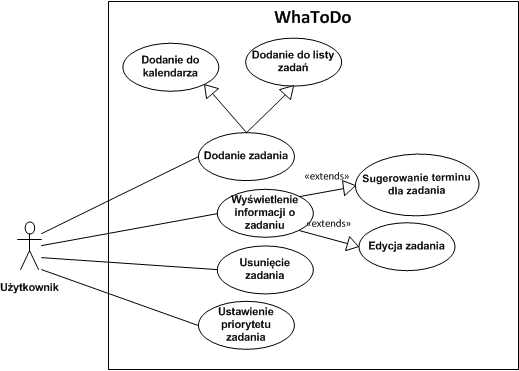
\includegraphics[width=\textwidth]{useCase}
\caption{Ogólny diagram przypadków użycia}
\label{fig:przypadki}
\end{figure}

Poniżej definicje trzech wybranych przypadków użycia.

\clearpage

\subsection{UC1: Dodanie zadania}

\textbf{Cel}: użytkownik chce dodać nowe zadanie

\textbf{Zdarzenie wyzwalające (trigger)}: użytkownik wybiera opcję Dodaj nowe zadanie

\textbf{Scenariusz główny}:
\begin{enumerate}
\item System wyświetla formularz wprowadzania informacji o zadaniu
\item Użytkownik wprowadza dane (nazwa, opis, czas trwania)
\item System zapisuje dane w bazie danych i odświeża widok (pojawia się nowe zadanie na liście zadań)
\end{enumerate}


\subsection{UC2: Zmiana priorytetu zadania}

\textbf{Cel}: użytkownik chce zmienić priorytet zadania

\textbf{Scenariusz główny}:
\begin{enumerate}
\item Użytkownik klika na zadanie i przeciąga je w odpowiednie miejsce (na listę zadań, co powoduje usunięcie priorytetu; na ćwiartkę obszaru roboczego - ustawienie ustalenie priorytetu)
\item System zapisuje zmiany w bazie danych
\end{enumerate}


\subsection{UC3: Sugerowanie terminu dla zadania}

\textbf{Cel}: użytkownik chce otrzymać od systemu propozycję terminu dla zadania z listy zadań

\textbf{Zdarzenie wyzwalające (trigger)}: użytkownik wybiera opcję \textit{Zasugeruj termin zadania}

\textbf{Scenariusz główny}:
\begin{enumerate}
\item System wyświetla propozycję terminu
\item Użytkownik akceptuje ją
\item System zapisuje zmiany w bazie danych
\end{enumerate}

\textbf{Scenariusz alternatywny}:
\begin{description}
\item[2A] Użytkownik nieakceptuje propozycji
\item[2A1] System oblicza inny dostępny termin
\item[2A2] Scenariusz główny jest kontynuowany od punktu 1.
\end{description}

\clearpage

\section{Baza danych}

\begin{figure}[!h]
\centering
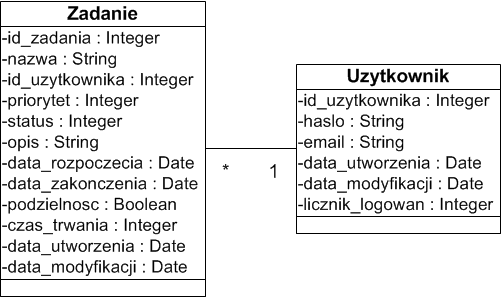
\includegraphics[width=.75\textwidth]{bazyDanych}
\caption{Schemat bazy danych}
\label{fig:bazaDanych}
\end{figure}


% ===========================================================================

\chapter{Metodyka pracy w naszej grupie}

\begin{enumerate}
\item \textit{Jaką metodykę pracy przyjęliśmy?}\\
Wzorowaliśmy się na metodykach zwinnych. Na nieregularnych spotkaniach, zarówno ,,przy piwie'', jak i za pośrednictwem internetu, omawialiśmy postępy, problemy i dalsze plany. Każdy podejmował się zadania, które uważał, że jest w stanie wykonać. W~przypadku problemów zgłaszaliśmy to w zespole i próbowaliśmy rozwiązać je wspólnie.

\item \textit{W jaki sposób się komunikowaliśmy?}\\
Główne ustalenia dotyczące projektu omawialiśmy na wspólnym spotkaniu przy stole i kartce papieru. Mniejsze uwagi odnośnie poprawy/zmiany/dodania funkcjonalności odnotowywaliśmy w specjalnie do tego celu stworzonym dokumencie na Google Docs. Pilne rozmowy przeprowadzane były za pośrednictwem czatu na Gmailu.

\item \textit{Jakie narzędzia wykorzystywaliśmy do synchronizacji?}\\
W celu synchronizacji tworzonego kodu, wykorzystaliśmy repozytorium założone w serwisie \texttt{github.com}

\end{enumerate}


% ===========================================================================

\chapter{Implementacja}

\section{Technologia}

\begin{itemize}
\item Cały nasz projekt został stworzony w środowisku \textbf{Netbeans}.
\item Aplikacja została oparta na frameworku \textbf{Ruby on Rails}. Wybór ten pociągnął za sobą dwie główne konsekwencje. Z jednej strony ułatwienie w postaci wymuszenia przez RoR korzystania z wzorca Model-View-Controller oraz w postaci dużej liczby dostępnych modułów i małej liczby potrzebnego kodu. Z drugiej strony było to dla nas dużym utrudnieniem, ponieważ nie mieliśmy wcześniej styczności zarówno z frameworkiem Ruby on Rails, jak i z samym językiem programowania Ruby. Należy tutaj zwrócić uwagę, że nie jest to framework prosty - dużo czasu zajęły nam próby zrozumienia jak on działa.
\item Wszystkie informacje o użytkownikach oraz zadaniach przechowywane są w bazie danych \textbf{PostgreSQL}.
\item Wykorzystano również fragment możliwości oferowanych przez \textbf{HTML5}. Konkretnie: tag \texttt{<details>} oraz natywny \textit{drag\&drop}.
\end{itemize}


\section{Moduły}

System składa się z czterech modułów:

\begin{itemize}
\item \textbf{Użytkownicy}. Odpowiedzialnego za zarządzanie użytkownikami serwisu: tworzenie i kasowanie kont.
\item \textbf{Autoryzacja}. Odpowiedzialnego za logowanie i wylogowywanie z aplikacji oraz utrzymywanie sesji.
\item \textbf{Zadania}. Odpowiedzialnego za tworzenie, edycję, kasowanie i przechowywanie zadań. Również za przydzielanie im priorytetów i proponowanie terminów realizacji (dla zadań, które nie mają ściśle określonego terminu).
\item \textbf{Kalendarz}. Odpowiedzialnego za wyświetlanie kalendarza, zawierającego zadania przesłane z modułu zadań.
\end{itemize}


\section{Algorytmy}

\subsection{Sugestia terminu dla wybranego zadania}
\label{sec:algJednoZadanie}

Algorytm otrzymuje na wejściu trzy parametry:
\begin{itemize}
\item \underline{zadanie} (w implementacji jest to konkretnie id zadania)
\item \underline{godzinę rozpoczęcia i zakończenia danego dnia} (\textit{godziny w których można przydzielać zadania; aktualnie są one narzucone z góry i zapisane bezpośrednio w kodzie; w przyszłości użytkownik miałby opcję określić te godziny dla każdego dnia tygodnia})
\item \underline{czas rozpoczęcia wyszukiwania} (\textit{opcjonalne; domyślnie algorytm rozpoczyna wyszukiwanie terminu dla zadania od ,,teraz''; tym parametrem można określić od jakiego terminu ma rozpocząć wyszukiwanie})
\end{itemize}

\begin{enumerate}
\item Jeżeli zadanie ma już określony termin: nic nie rób.
\item Jeżeli zadanie jest dłuższe od jednego dnia roboczego: nic nie rób (\textit{algorytm w podstawowej wersji nie ma możliwości podziału zadań na mniejsze części - planowaliśmy to wprowadzić w kolejnej wersji}).
\item Ustal \underline{czas startu} na \underline{czas rozpoczęcia wyszukiwania}, jeżeli ustawiony, w przeciwnym przypadku na aktualny czas. Ustal \underline{czas zakończenia} na \underline{czas startu}+\underline{czas trwania}.
\item Jeżeli \underline{czas zakończenia} jest późniejszy od \underline{deadline'u}, zwróć informację o niepowodzeniu i zakończ algorytm.
\item Pobierz wszystkie zadania z ustalonym czasem rozpoczęcia i zakończenia
\item Weź pierwsze zadanie z pobranej listy i sprawdź czy jego termin zachodzi na zakres \underline{czas startu}-\underline{czas zakończenia}.
\item Jeżeli terminy na siebie zachodzą, ustal \underline{czas rozpoczęcia wyszukiwania} na czas zakończenia zadania znalezionego w bazie i rozpocznij algorytm od początku.
\item Jeżeli terminy na siebie nie zachodzą i są jeszcze jakieś zadania na liście, wróć do punktu~6.
\item Przedstaw ustalony termin do akceptacji użytkownikowi.
\item W przypadku braku akceptacji, powtórz algorytm. Ustaw \underline{czas rozpoczęcia wyszukiwania} na \underline{czas startu}+1 godzina (\textit{1 godzina została wybrana przez nas i nie ma żadnego uzasadnienia. Powoduje tylko i wyłącznie zaproponowanie późniejszego terminu rozpoczęcia zadania}).
\item W przypadku akceptacji, zapisz informacje w bazie.
\end{enumerate}

\subsection{Sugestia planu na najbliższy tydzień}
\label{sec:algPlanTygodniowy}

\textit{Algorytm ten nie został zaimplementowany z powodu braku czasu (i początkowo braku umiejętności programowania w Ruby). Tutaj przedstawiamy wersję, którą planowaliśmy zaimplementować w pierwszej wersji aplikacji.}

\begin{enumerate}
\item Pobierz listę wszystkich zadań, które nie mają ustalonego terminu.
\item Posortuj listę najpierw wg priorytetów: 1. Ważne-pilne 2. Nieważne-pilne 3. Ważne-niepilne 4. Nieważne-niepilne 5. Bez priorytetu, a następnie wg deadline (od najbliższego do najpóźniejszego).
\item Weź pierwsze zadanie z listy i szukaj dla niego propozycji terminu (\textit{wg algorytmu z sekcji~\ref{sec:algJednoZadanie}}).
\item Zapisz w lokalnej tablicy propozycję terminu dla tego zadania (tablica indeksowana po id tasków).
\item Powtórz kroki 3 i 4 do wyczerpania listy zadań, bądź do wyczerpania czasu w tygodniu.
\item Zaprezentuj znalezione terminy użytkownikowi.
\item W przypadku braku akceptacji, powtórz algorytm. Tym razem dla pierwszego zadania wywołaj algorytm sugestii terminu z ustawionym \underline{czasem rozpoczęcia wyszukiwania} na \texttt{teraz + random(1:24) godzin} (dzięki temu zostaną przedstawione inne propozycje).
\item W przypadku akceptacji, zapisz informacje w bazie.
\end{enumerate}


\section{Warstwa Prezentacji}

TODO: Tutaj krótki opis i kilka zrzutów ekranu

%\begin{figure}[!h]
%\centering
%\includegraphics[width=\textwidth]{Prezentacja1}
%\caption{Schemat procesu implementacji}
%\label{schematProcesuImplementacji}
%\end{figure}

% ===========================================================================

\chapter{Podsumowanie}

\section{Co udało się zrealizować?}

TODO: Czy jesteśmy zadowoleni i takie tam.

\section{Napotkane problemy}

TODO: Chociażby to, że Ruby jest dla nas nieznaną technologią.

\section{Możliwości dalszego rozwoju projektu}

TODO: Trzeba zaglądnąć w listę rzeczy, które mamy w specyfikacji i jakoś opisać + może mamy jakieś inne pomysły jeszcze ;)

\section{Promocja i reklama}

Portal nazwaliśmy ,,whaTodo'', co jest skrótem od angielskiego ,,what to do''. Nazwa ta wskazuje na główną innowację naszej aplikacji czyli sugerowanie terminów wykonywania zadań, które nie mają ściśle określonego czasu wykonania.

Po dopracowaniu serwisu i zakupieniu domeny, chcieliśmy go udostępnić dla wszystkich zainteresowanych. W ramach promocji naszego serwisu przez pierwszy miesiąc dostęp do wszystkich funkcjonalności byłby darmowy. W kolejnych miesiącach zakładaliśmy użytkowanie aplikacji za symboliczne 2 zł / miesiąc.

Hasło reklamowe: ,,\textbf{Nie wiesz za które zadanie się teraz zabrać? Wejdź na www.whatodo.pl i pozwól sobie
pomóc!}''

\end{document}

